\section{Podzadanie C}
\subsection{Analiza danych}
\subsubsection{Rozkład wartości etykiety}

Podzadanie C dotyczyło podobieństwa nowych pytań do istniejących komentarzy.  Każdy komentarz w zbiorze zawierał etykietę RELC\_RELEVANCE2ORGQ, która określała to podobieństwo. Etykieta przyjmowała trzy wartości: ,,Good'', ,,PotentiallyUseful'' oraz ,,Bad''. Rozkład etykiet w oryginalnym zbiorze przedstawiono w tablicy~\ref{c_original_set_percentage}.

\begin{table}[H]
\caption{Rozkład ilościowy klas w oryginalnym zbiorze.}
\label{c_original_set_percentage}
    \begin{center}
        \begin{tabular}{ |c|c| } 
            \hline
            ,,Good'' & 9,95\% \\
            \hline
            ,,PotentiallyUseful'' & 8,44\% \\
            \hline
            ,,Bad'' & 81,61\% \\ 
            \hline
        \end{tabular}
    \end{center}
\end{table}

Ze względu na sprowadzenie problemu do decyzji binarnej, klasa ,,PotentiallyUseful'' była traktowana jako część klasy ,,Good''. Tablica \ref{c_merged_set_percentage} pokazuje rozkład po złączeniu klas.

\begin{table}[H]
\caption{Rozkład ilościowy klas po połączeniu.}
\label{c_merged_set_percentage}
    \begin{center}
        \begin{tabular}{ |c|c| } 
            \hline
            ,,Good'' & 18,39\% \\
            \hline
            ,,Bad'' & 81,61\% \\ 
            \hline
        \end{tabular}
    \end{center}
\end{table}

\subsubsection{Sprawdzenie podobieństwa dla podstawowych miar}

Kolejnym etapem analizy danych było sprawdzenie powiązania między wartościami podstawowych miar podobieństwa a faktycznym podobieństwem, które było opisane w zbiorze danych za pomocą etykiety.

Rysunek~\ref{c_jaccard_distance} przedstawia medianę odległości Jaccarda dla obu klas w zbiorze. Dodatkowo na wykresie widać wartość pierwszego i trzeciego kwartyla oraz minimum i maksimum przyjmowanych wartości.

\begin{figure}[H]
\centering
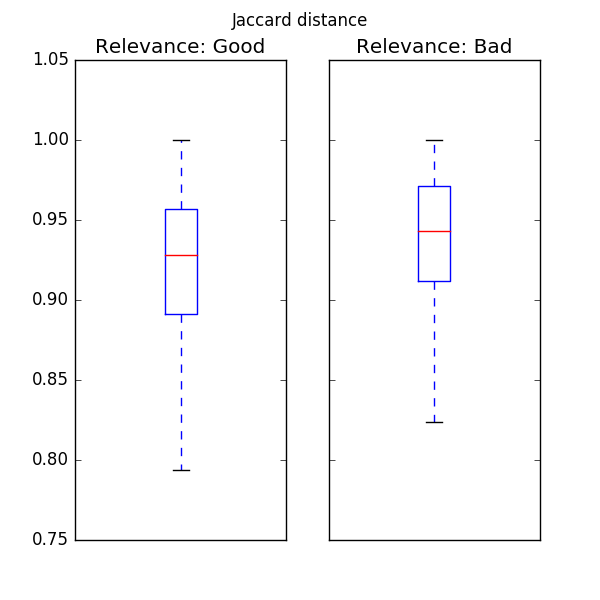
\includegraphics[scale=0.5]{c_Jaccard_distance.png}
\caption{Odległość Jaccarda.}
\label{c_jaccard_distance}
\end{figure}

Niestety otrzymane wyniki nie pozwalają na wyznaczenie wartości odległości Jaccarda, która oddzieliłaby skutecznie obie klasy. Miara ta bada podobieństwo jedynie na podstawie liczby tych samych słów użytych w porównywanych tekstach. Przykłady z klasy ,,Bad'', mimo różnicy znaczeniowej pytań i komentarzy, otrzymują wysokie wyniki, ponieważ w tekstach pojawiają się te same słowa.

Kolejną badaną miarą było podobieństwo cosinusowe. Wyniki przedstawia rysunek~\ref{c_cosine_similarity}.

\begin{figure}[H]
\centering
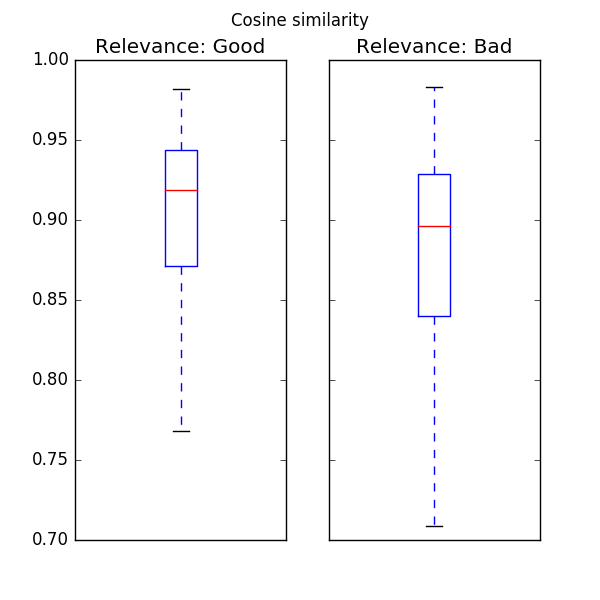
\includegraphics[scale=0.5]{c_Cosine_similarity.png}
\caption{Podobieństwo cosinusowe.}
\label{c_cosine_similarity}
\end{figure}

Choć w tym przypadku rozbieżność mediany dla klas jest nieco większa, nadal nie jest możliwe jednoznaczne rozdzielenie ze względu na podobne rozstępy międzykwartylowe. Wartości ponownie rozkładają się zbyt blisko siebie.

Rysunek~\ref{c_length_difference} przedstawia wyniki dla prostego badania różnicy długości.

\begin{figure}[H]
\centering
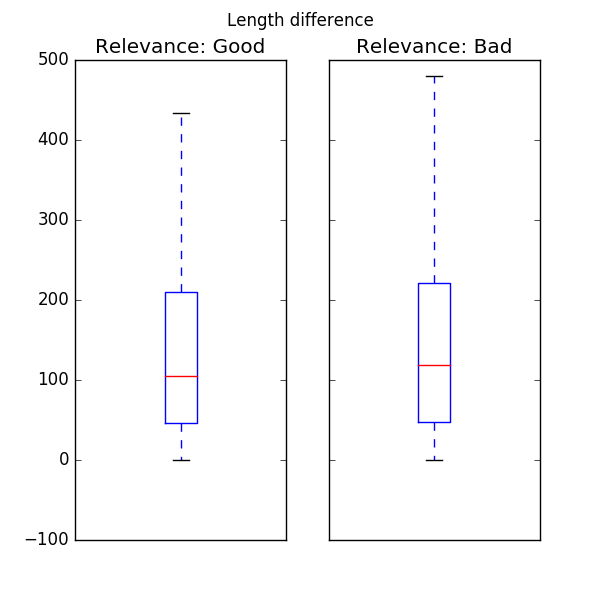
\includegraphics[scale=0.5]{c_Length_difference.png}
\caption{Różnica długości.}
\label{c_length_difference}
\end{figure}

W przypadku tej miary ponownie widać duże podobieństwo wyników dla obu klas. Wyniki pozwalają wręcz wnioskować, że w całym zbiorze danych różnica długości dla między pytaniem a komentarzem oscyluje w granicach 100 znaków. Niestety dla badania pobobieństwa miara różnicy długości nie była pomocna.

\subsection{Reprezentacja w postaci word embeddingów}
Ze względu na niską skuteczność podstawowych miar postanowiono użyć bardziej złożonych modeli klasyfikujących -- sieci neuronowych. Aby w pełni wykorzystać możliwości sieci do znajdowania wzorców, jako reprezentacje słów zostały wykorzystane \textit{word embeddingi}. Użyto zbioru wektorów udostępnianego przez firmę Google.

\subsection{Prosta sieć neuronowa (feed-forward)}

Pierwszy model sieci neuronowej jaki został przetestowany opierał się na prostej architekturze z jedną warstwą ukrytą o rozmiarze 128 jednostek. Ponieważ przygotowane próbki danych składały się z par pytanie-odpowiedź, sieć posiadała dwa wejścia. Każde z wejść było połączone z warstwą \textit{embedding}, czyli warstwą konwertującą dane wejściowe na reprezentacje wektorowe. Wektory wyjściowe były następnie łączone w jeden w warstwie konkatenacji. Połączony wektor trafiał do warstwy prostej, złożonej ze 128 neuronów. Ostatnią warstwę stanowił pojedynczy neuron wyjściowy.

Tak zbudowaną sieć wytrenowano w procesie trwającym 400 epok. Rysunki~\ref{c_feedforward_acc} oraz \ref{c_feedforward_loss} przedstawiają uzyskane wyniki.

\begin{figure}[H]
\centering
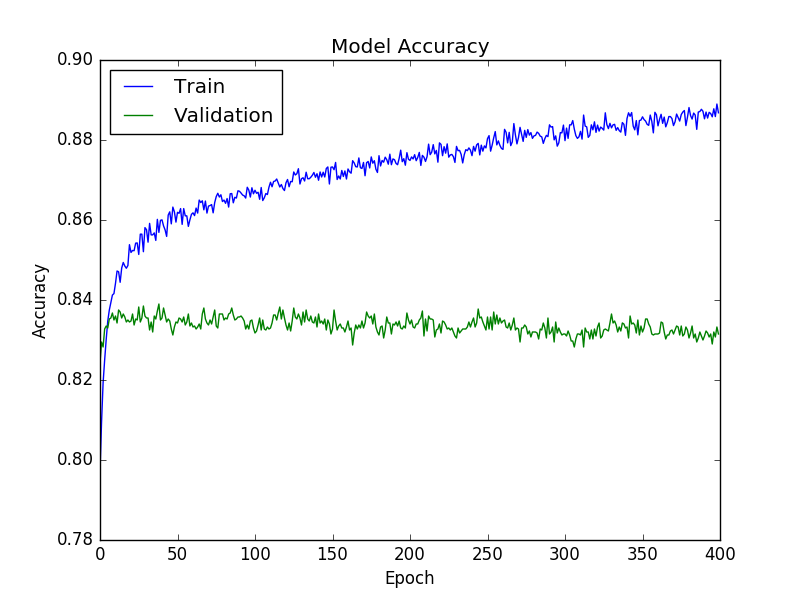
\includegraphics[scale=0.5]{c_feedforward_1_dense_128_acc.png}
\caption{Trafność sieci prostej.}
\label{c_feedforward_acc}
\end{figure}

\begin{figure}[H]
\centering
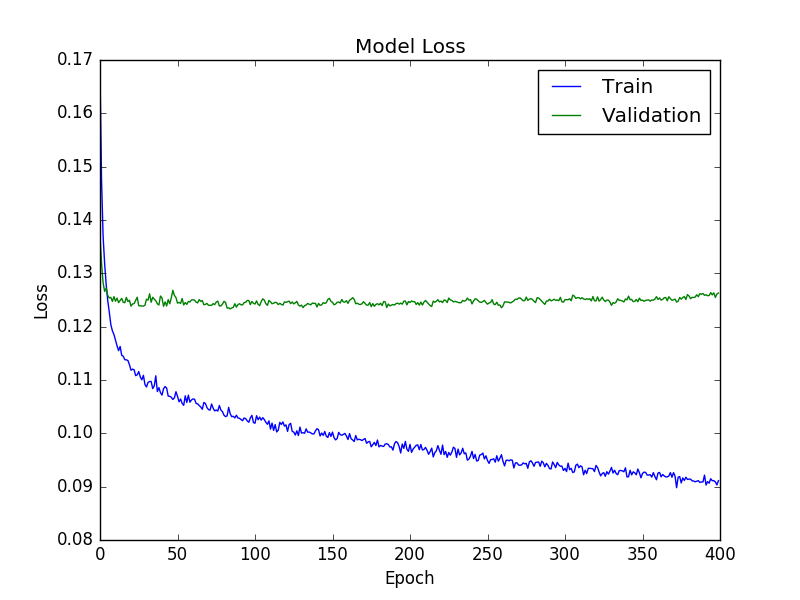
\includegraphics[scale=0.5]{c_feedforward_1_dense_128_loss.png}
\caption{Strata sieci prostej.}
\label{c_feedforward_loss}
\end{figure}

Choć na zbiorze trenującym sieć osiąga wysoką trafność, a błąd jest niewielki, na zbiorze walidującym wyniki nie ulegają znacznej poprawie w trakcie uczenia. Zarówno trafność jak i strata oscylują w granicach wartości uzyskanych w początkowych etapach treningu. W przypadku trafności można zauważyć nawet trend spadkowy. Są to objawy przeuczenia sieci, czyli zbyt silnego uzależnienia od przypadków ze zbioru trenującego.

\subsection{Sieci rekurencyjne}
\subsubsection{Sieć LSTM}

Zostały wytrenowane dwa modele sieci oparte o warstwę rekurencyjną \emph{Long Short-Term Memory} (LSTM). Warstwa w obu przypadkach miała rozmiar 128 jednostek. Model pierwszy składał się dodatkowo z warstwy prostej o tej samej wielkości i z jednego neuronu stanowiącego wyjście sieci. Wyniki przedstawiają rysunki~\ref{c_lstm_1_acc} oraz \ref{c_lstm_1_loss}.

\begin{figure}[H]
\centering
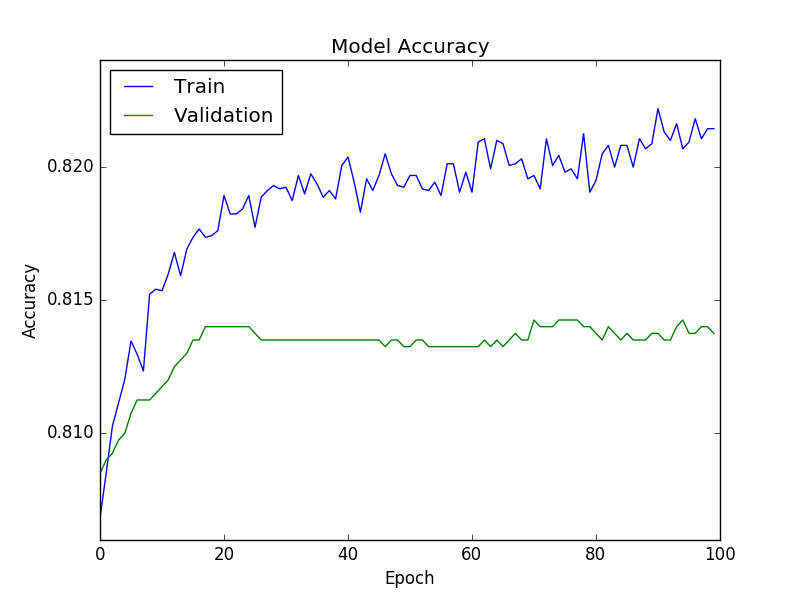
\includegraphics[scale=0.5]{c_lstm_1_dense_acc.png}
\caption{Trafność pierwszego modelu.}
\label{c_lstm_1_acc}
\end{figure}

\begin{figure}[H]
\centering
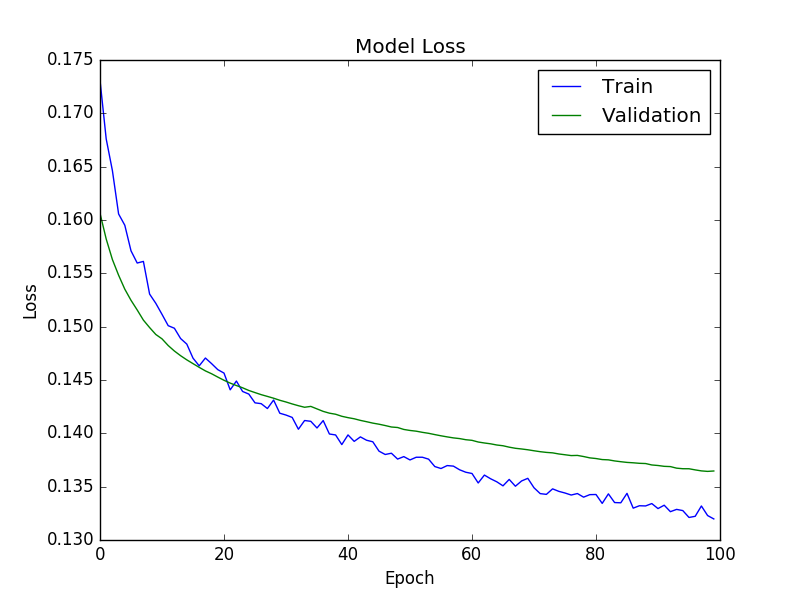
\includegraphics[scale=0.5]{c_lstm_1_dense_loss.png}
\caption{Strata pierwszego modelu.}
\label{c_lstm_1_loss}
\end{figure}

Wyniki wskazują na lekką poprawę w porównaniu z siecią prostą. Po wprowadzeniu warstwy rekurencyjnej sieć osiąga wynik trafności w granicach 81,5\% i nie wykazuje trendu spadkowego w trakcie uczenia. Mimo, że trafność na zbiorze trenującym jest nieco wyższa, strata modelu na obu zbiorach jest zbliżona i zachowała trend malejący. Sieć oparta na jednej warstwie prostej i jednej warstwie rekurencyjnej nie została przeuczona.

Model drugi wykorzystywał poza warstwą rekurencyjną, dwie warstwy proste o rozmiarach 128 i 64 jednostek oraz pojedynczy neuron wyjściowy. Wyniki uczenia przedstawiono na rysunkach~\ref{c_lstm_2_acc} oraz \ref{c_lstm_2_loss}.

\begin{figure}[H]
\centering
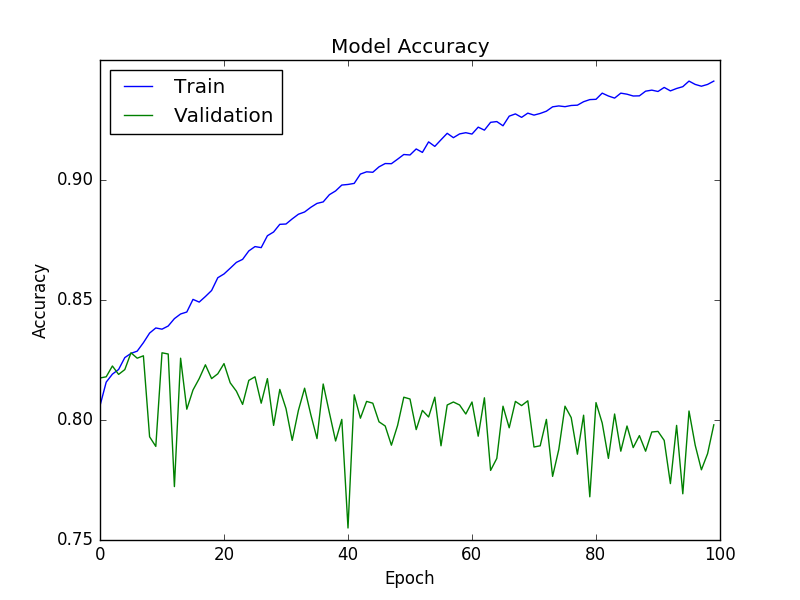
\includegraphics[scale=0.5]{c_lstm_3_dense_acc.png}
\caption{Trafność drugiego modelu.}
\label{c_lstm_2_acc}
\end{figure}

\begin{figure}[H]
\centering
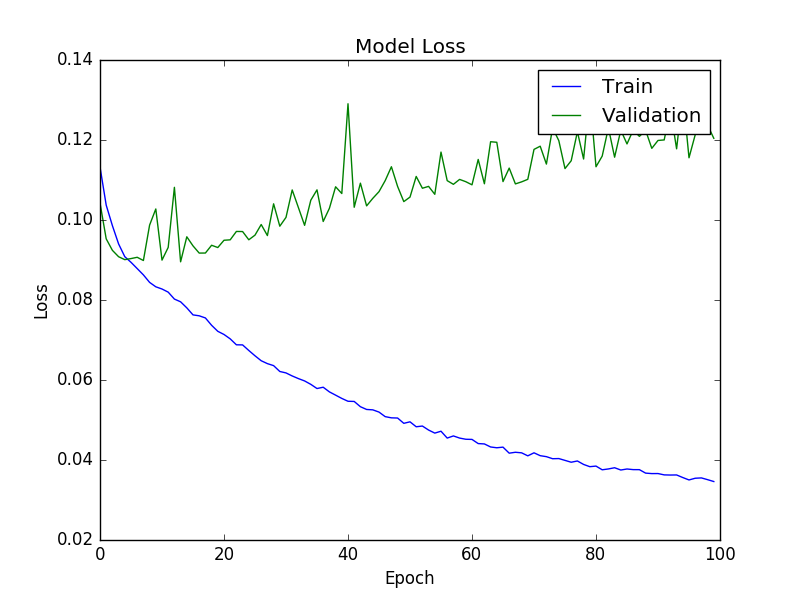
\includegraphics[scale=0.5]{c_lstm_3_dense_loss.png}
\caption{Strata drugiego modelu.}
\label{c_lstm_2_loss}
\end{figure}

Choć po kilku pierwszych epokach model ma zbliżone wyniki na obu zbiorach, szybko następuje przeuczenie. Na zbiorze walidującym trafność spada, a strata rośnie. Prawdopodobnie jest to spowodowane wprowadzeniem dodatkowej warstwy prostej. Po analizie wyników dla sieci feed-forward można wnioskować, że to tego typu warstwy są wrażliwe na przeuczenie. Aby uzyskać model nieprzeuczony, osiągający skuteczność ok. 82\% należałoby zatrzymać proces uczenia już po pięciu epokach.

\subsubsection{Sieć MaLSTM}
W celu dalszego poprawienia wyników stworzona została sieć syjamska w wariancie ogólnym. Model składał się z dwóch podsieci zawierających po jednej warstwie rekurenyjnej Long Short-Term Memory. Każda z nich o rozmiarze 128 jednostek. Dla wektorów na wyjściach obu podsieci była następnie obliczana norma w metryce manhatańskiej. Obliczona wartość trafiała do pojedynczego neuronu, który stanowił wyjście sieci.

Wyniki dot. trafności i straty przedstawiają rysunki~\ref{c_siamese_acc} i \ref{c_siamese_loss}.

\begin{figure}[H]
\centering
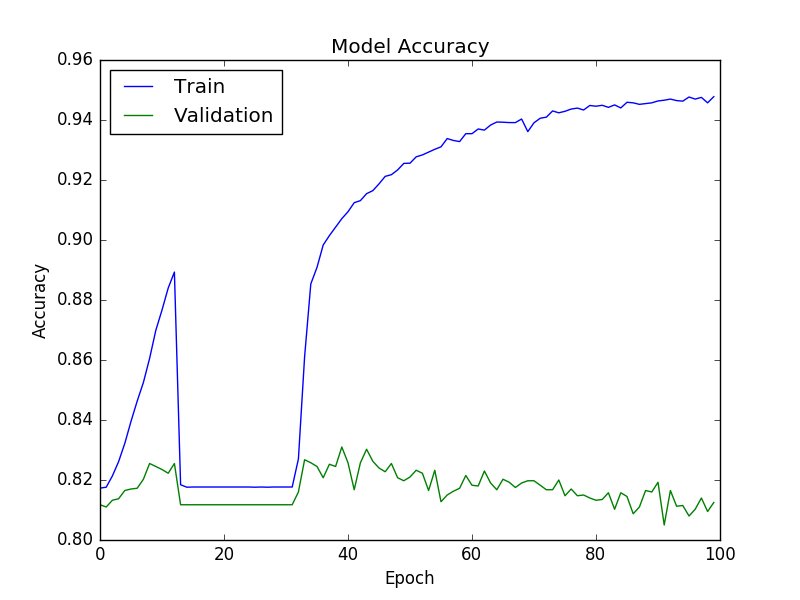
\includegraphics[scale=0.5]{c_malstm_org_dataset_acc.png}
\caption{Trafność sieci syjamskiej.}
\label{c_siamese_acc}
\end{figure}

\begin{figure}[H]
\centering
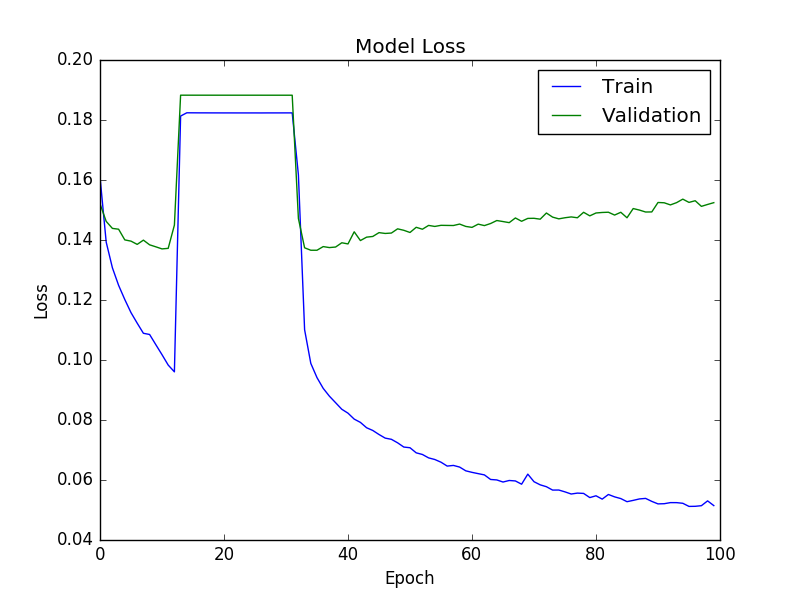
\includegraphics[scale=0.5]{c_malstm_org_dataset_loss.png}
\caption{Strata sieci syjamskiej.}
\label{c_siamese_loss}
\end{figure}

Wyraźnie widać, że w trakcie uczenia wystąpiła anomalia. Od epoki 15, przez ok. 20 epok zarówno trafność jak i strata na obu zbiorach mają stałe wartości. Prawdopodobnie przez ten okres wartości wag nie były w ogóle zmieniane. W dalszej części uczenia widać, że po raz kolejny wystąpiło przeuczenie, ponieważ mimo wzrostu trafności na zbiorze trenującym, trafność na zbiorze walidującym spadała. Podobnie strata, choć malała na zbiorze trenującym, rosła w przypadku zbioru walidującego. W najlepszym momencie sieć syjamska osiągnęła wynik niewiele ponad 82\% trafności.

\subsubsection{Rozszerzenie zbioru danych}

Jednym ze sposobów poprawy skuteczności modelu jest wytrenowanie go na większym zbiorze danych. W przypadku zbiorów dla uczenia nadzorowanego, warto również zwrócić uwagę na rozkład ilościowy poszczególnych klas. Dla podzadania C rozkład nie jest równy, ponieważ około 80\% przypadków należy do tej samej klasy.

Na podstawie oryginalnego zbioru został stworzony zbiór rozszerzony, w którym nowe próbki utworzono zamieniając niektóre wyrazy na ich synonimy. Dodatkowo, w celu wyrównania liczności klas, rozszerzeniu podlegały tylko próbki należące do klasy ,,Good''. Dokładną charakterystykę zbioru oryginalnego i rozszerzonego przedstawia tablica~\ref{c_augmented_set_percentage}.

\begin{table}[H]
\caption{Rozkłady ilościowe klas w zbiorze oryginalnym i rozszerzonym.}
\label{c_augmented_set_percentage}
    \begin{center}
        \begin{tabular}{ |c|c|c|c| } 
            \hline
            Zbiór & Liczność zbioru & ,,Good'' & ,,Bad''\\
            \hline
            Oryginalny & 19954 & 18,38\% & 81,61\%\\
            \hline
            Rozszerzony & 40370 & 59,66\% & 40,34\%\\ 
            \hline
        \end{tabular}
    \end{center}
\end{table}

Na zbiorze rozszerzonym został wytrenowany model sieci syjamskiej. Wyniki przedstawiają rysunki~\ref{c_siamese_augmented_acc} i \ref{c_siamese_augmented_loss}.

\begin{figure}[H]
\centering
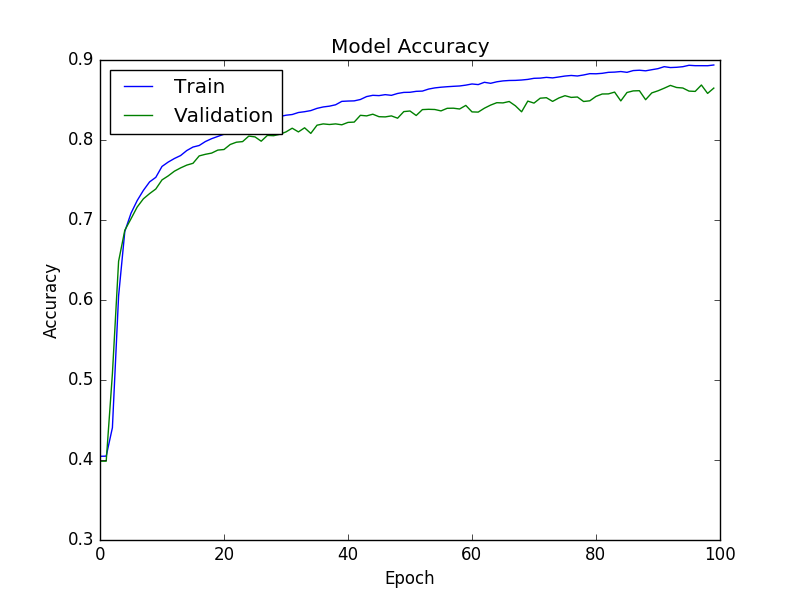
\includegraphics[scale=0.5]{c_siamese_augmented_dataset_acc.png}
\caption{Trafność sieci syjamskiej na zbiorze rozszerzonym.}
\label{c_siamese_augmented_acc}
\end{figure}

\begin{figure}[H]
\centering
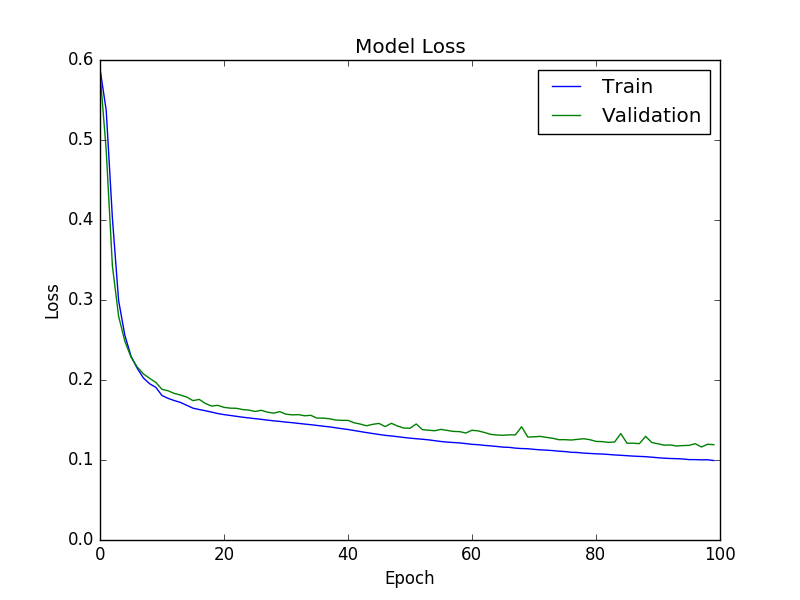
\includegraphics[scale=0.5]{c_siamese_augmented_dataset_loss.png}
\caption{Strata sieci syjamskiej na zbiorze rozszerzonym.}
\label{c_siamese_augmented_loss}
\end{figure}

Trafność działania modelu na zbiorze walidującym została zwiększona, osiągnęła ostatecznie wynik około 85\%.

\subsection{Ocena rezultatów}
Warto rozważyć otrzymane wyniki w oparciu o rozkład danych. W zbiorze oryginalnym ok. 80\% stanowiły przykłady z klasy ,,Bad''. Oznacza to, że klasyfikator, który dla każdej pary pytanie-odpowiedź zwracałby klasę ,,Bad'' osiągałby poziom trafności w granicach 80\%. Model sieci syjamskiej wytrenowany na oryginalnym zbiorze osiągnął trafność ok. 82\%. Wynik ten, choć na pierwszy rzut oka wysoki, nie przewyższa zanadto wyniku, który mógłby osiągnąć naiwny klasyfikator zwracający zawsze tą samą klasę. Poprawę trafności widać dopiero po wytrenowaniu tej samej sieci syjamskiej na zbiorze rozszerzonym. W tej wersji zbioru rozkład klas jest bardziej równomierny, naiwny klasyfikator mógłby osiągnąć na nim co najwyżej trafność ok. 60\%, ponieważ taką część zbioru stanowi klasa ,,Good''. Sieć syjamska osiąga trafność na poziomie 85\%.